<<<<<<<<<<\documentclass[a4paper, 10pt, fleqn]{article}

\usepackage[utf8]{inputenc}
\usepackage[T1]{fontenc}
\usepackage{textcomp}
\usepackage{lmodern}
\usepackage[ngerman]{babel}
\usepackage{tocbibind}
\usepackage{enumerate}
\usepackage[table]{xcolor}
\usepackage{pdfpages}
\usepackage{amsmath}
\usepackage{graphicx}
\usepackage{geometry}
\usepackage{scrpage2}
\usepackage{lastpage}
\usepackage[hyphens]{url}
\usepackage{hyperref}
\usepackage{listings}
\usepackage{float}
\restylefloat{figure}
\lstset{language=[ansi]C++}

\newcommand{\code}[1]{\texttt{#1}}

\renewcommand*{\listoffigures}{%
  \begingroup
  \tocchapter
  \tocfile{\listfigurename}{lof}
  \endgroup
}

\geometry{left=3cm, top=3cm, bottom=3cm, right=2cm}

\hypersetup{
    colorlinks,
    linkcolor=black,
    citecolor=black,
    urlcolor=black
}

\pagestyle{scrheadings}
\ihead{APPE Team 13}\ohead{Systemspezifikation} 
\ifoot{\today} \ofoot{Seite \thepage\ von {\hypersetup{linkcolor=black}\pageref{LastPage}}}

% Einrücken zu Beginn von neuem Absatz unterdrücken
\setlength{\parindent}{0pt}

% Zeilenabstand einstellen
\usepackage{setspace}
\makeatletter
\newcommand{\MSonehalfspacing}{%
  \setstretch{1.44}%  default
  \ifcase \@ptsize \relax % 10pt
    \setstretch {1.448}%
  \or % 11pt
    \setstretch {1.399}%
  \or % 12pt
    \setstretch {1.433}%
  \fi
}
\newcommand{\MSdoublespacing}{%
  \setstretch {1.92}%  default
  \ifcase \@ptsize \relax % 10pt
    \setstretch {1.936}%
  \or % 11pt
    \setstretch {1.866}%
  \or % 12pt
    \setstretch {1.902}%
  \fi
}
\makeatother
\MSonehalfspacing


\begin{document}

% !TEX root = Dokumentation.tex
\begin{titlepage}   

\begin{center}
\textsc{\Large Team 13}\\[0.5cm]

% Title
\newcommand{\HRule}{\rule{\linewidth}{0.5mm}}
\HRule \\[0.4cm]
{ \huge \bfseries Filialbestellsystem}\\[0.4cm]
{ \LARGE \bfseries Projektmanagementplan}\\[0.4cm]
\HRule \\[1.5cm]

% Unterer Teil der Seite
{\large Rotkreuz, \today}

\begin{figure}[H]%Position festigen
\centering
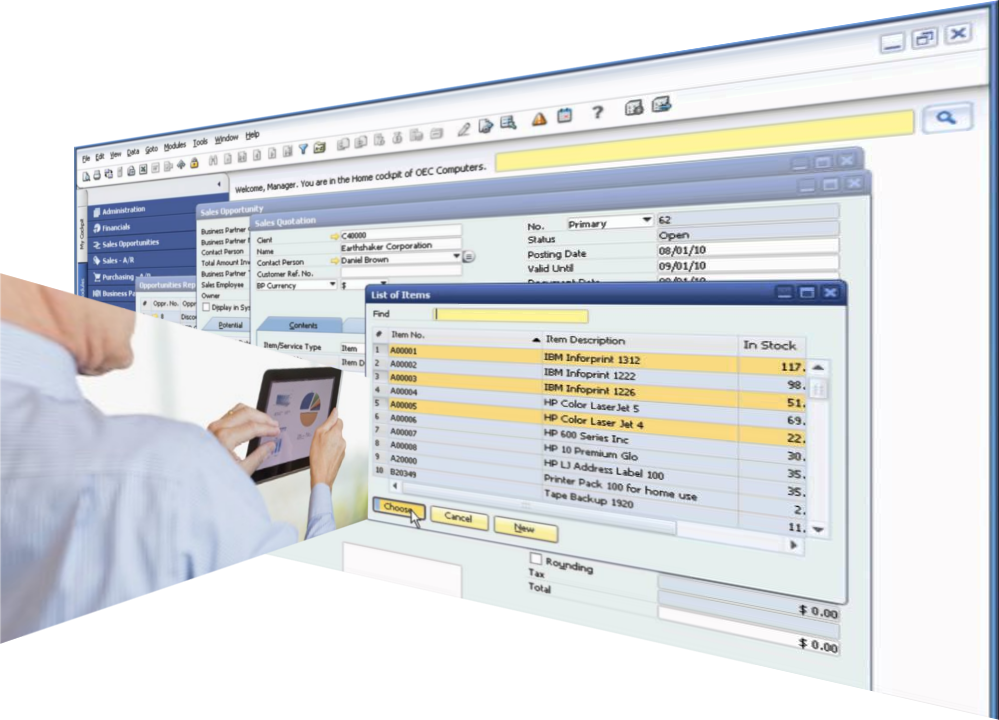
\includegraphics[width=0.7\textwidth]{Images/Titelbild.png}
\label{fig:title}
\end{figure}
% Author and supervisor
\begin{minipage}{0.4\textwidth}
\begin{flushleft} \large
\emph{Autoren:}\\
Marco Moro\\
Severin Gmür\\
Ramon Wyss\\
Tobias Kreienbühl\\
\end{flushleft}
\end{minipage}
\hfill
\begin{minipage}{0.4\textwidth}
\begin{flushright} \large
%\emph{Supervisor:} \\
%tbd
\end{flushright}
\end{minipage}
\large
\vfill
I.BA\_APPE.F1701 \\
Hochschule Luzern Informatik

\end{center}

\end{titlepage}
\tableofcontents
\clearpage
\section{Systemübersicht}

\section{Use Case}
%-------------------
% Use Case
%-------------------
% !TEX root = Dokumentation_SysSpec.tex
\subsection{Use Case Übersicht}
%--------------------------
% Bild Übersicht
%--------------------------

\begin{figure}[H]%Position festigen
\centering
\includegraphics[width=0.7\textwidth]{Images/usecase-u.png}
\label{fig:usecase}
\end{figure}


\subsection{Use Case Beschreibung}
In diesem Abschnitt wird die unter Abbildung 2 dargestellte Use Case Übersichtlich tabellarisch genauer beschrieben.

%--------------------------
%Tabellen usecase/1usecase
%--------------------------
% !TEX root = Dokumentation_SysSpec.tex
\subsubsection{Use Case 1: Anmeldung}
\begin{table}[H]
\begin{tabular}{ | p{0.22\textwidth} | p{0.68\textwidth} |} \hline
\rowcolor{gray!50}
%Titelzeile
	\textbf{Name}          &
	\begin{tabular}{l}
		\textbf{Anmeldung}
	\end{tabular}
	\\ \hline
%Zeile
	\textbf{Kurzbeschreibung}			 &
	\begin{tabular}{l}
		Ein Benutzer meldet sich im System an
	\end{tabular}
\\ \hline
%Zeile
	\textbf{Akteure}}   		 &
	\begin{tabular}{l}
		Filialleiter, Verkaufspersonal, Sysadmin, Filialverwalter, Datatypist
	\end{tabular}
\\ \hline
%Zeile
	\textbf{Auslöser}              & 
	\begin{tabular}{l}
		Der Akteure will sich am System anmelden
	\end{tabular}
\\ \hline
%Zeile
	\textbf{Vorbedingungen}       &
	\begin{tabular}{l}
		-	Der Akteur muss im System vorhanden sein \\
		-	Benutzername muss vorhanden sein \\
		-	Passwort muss vorhanden sein \\

	\end{tabular}		
\\ \hline
%Zeile
	\textbf{Input Information}             &        
	\begin{tabular}{l}
		-	Username \\
		-	Passwort

	\end{tabular}
\\ \hline
%Zeile
	\textbf{Ergebnisse}  &
	\begin{tabular}{l}
		Benutzer ist am System angemeldet.
	\end{tabular}
\\ \hline
%Zeile
	\textbf{Nachbedingung}				 &
	\begin{tabular}{l}
		Benutzer kann im System je nach definierter Rolle arbeiten.
	\end{tabular}
\\ \hline
%Zeile
	\textbf{Ablauf}            &
	\begin{tabular}{l}
		1.	Applikation starten \\
		2.	Username \& Passwort eingeben \\
		3.	Schaltfläche \glqq{} \«Login\»\grqq{} betätigen

	\end{tabular}
\\ \hline
%Zeile
	\textbf{Sonderfälle}			 &
	\begin{tabular}{l}
		Passwort wird 3-mal falsch eingegeben.
	\end{tabular}
\\ \hline	
%Untere Abgrenzung
\end{tabular}
\end{table}
% !TEX root = Dokumentation_SysSpec.tex
\subsubsection{Use Case 2:Bestellung einsehen }
\begin{table}[H]
\begin{tabular}{ | p{0.22\textwidth} | p{0.68\textwidth} |} \hline
\rowcolor{gray!50}
%Titelzeile
	\textbf{Name}          &
	\begin{tabular}{l}
		\textbf{Bestellung einsehen}
	\end{tabular}
	\\ \hline
%Zeile
	\textbf{Kurzbeschreibung}			 &
	\begin{tabular}{l}
		Akteure kann sich alle offenen Bestellungen ansehen.
	\end{tabular}
\\ \hline
%Zeile
	\textbf{Akteure}   		 &
	\begin{tabular}{l}
		Filialleiter, Verkaufspersonal
	\end{tabular}
\\ \hline
%Zeile
	\textbf{Auslöser}              & 
	\begin{tabular}{l}
		Ein Akteure will die Bestellungen einsehen.
	\end{tabular}
\\ \hline
%Zeile
	\textbf{Vorbedingungen}       &
	\begin{tabular}{l}
		-	Der Akteur muss im System angemeldet sein
	
	\end{tabular}		
\\ \hline
%Zeile
	\textbf{Input Information}             &        
	\begin{tabular}{l}
		-	Auswahl aus Liste.

	\end{tabular}
\\ \hline
%Zeile
	\textbf{Ergebnisse}  &
	\begin{tabular}{l}
		Bestellung wird angezeigt.
	\end{tabular}
\\ \hline
%Zeile
	\textbf{Nachbedingung}				 &
	\begin{tabular}{l}
		-
	\end{tabular}
\\ \hline
%Zeile
	\textbf{Ablauf}            &
	\begin{tabular}{l}
		1.	Bestellung aus Liste auswählen. \\
		2.	Doppelklick auf anzuzeigende Bestellung.

	\end{tabular}
\\ \hline
%Zeile
	\textbf{Sonderfälle}			 &
	\begin{tabular}{l}
		-
	\end{tabular}
\\ \hline	
%Untere Abgrenzung
\end{tabular}
\label{tab:2usecase}
\caption{Use Case 2: Bestellung einsehen}
\end{table}
% !TEX root = Dokumentation_SysSpec.tex
\subsubsection{Use Case 3: Bestellung erfassen}
\begin{table}[H]
\begin{tabular}{ | p{0.22\textwidth} | p{0.68\textwidth} |} \hline
\rowcolor{gray!50}
%Titelzeile
	\textbf{Name}          &
	\begin{tabular}{l}
		\textbf{Bestellung erfassen}
	\end{tabular}
	\\ \hline
%Zeile
	\textbf{Kurzbeschreibung}			 &
	\begin{tabular}{l}
		Ein Akteure erfasst aus den bestehenden Produkten eine Bestellungen.
	\end{tabular}
\\ \hline
%Zeile
	\textbf{Akteure}   		 &
	\begin{tabular}{l}
		Filialleiter, Verkaufspersonal
	\end{tabular}
\\ \hline
%Zeile
	\textbf{Auslöser}              & 
	\begin{tabular}{l}
		Kunde möchte via Akteure ein Produkt bestellen.
	\end{tabular}
\\ \hline
%Zeile
	\textbf{Vorbedingungen}       &
	\begin{tabular}{l}
		-	Der Akteur muss im System angemeldet sein (Use Case 1 erfüllt).\\
		-	Der Akteur ist berechtige Bestellungen zu erfassen. \\
		- 	Der Kunde muss bereits im System erfasst sein \\
		- 	Das Produkt muss in der Datenbank (Filliallager) vorhanden sein. 
  

	\end{tabular}		
\\ \hline
%Zeile
	\textbf{Input Information}             &        
	\begin{tabular}{l}
		
		-   Kunde \\
		-	Produkt \\
		-  	Anzahl 
		

	\end{tabular}
\\ \hline
%Zeile
	\textbf{Ergebnisse}  &
	\begin{tabular}{l}
		Verkäufer erfasst von Kunde gewünschte Produkte.
	\end{tabular}
\\ \hline
%Zeile
	\textbf{Nachbedingung}				 &
	\begin{tabular}{l}
		Wenn Bestellung erfasst ist, wird Rechnungswesen benachrichtigt \& \\
		der Kunde erhält eine Bestellbestätigung.
	\end{tabular}
\\ \hline
%Zeile
	\textbf{Ablauf}            &
	\begin{tabular}{l}
		1.	Verkäufer ist am System angemeldet. \\
		2.	Kunde auswählen (Dropdown List). \\
		3.  Produkt in Liste suchen und Anzahl eingeben.\\
		4.  Falls mehrere Produkte gewünscht werden, Schritt 3 wiederholen.\\
		5.	Schaltfläche \grqq Bestellung absenden\grqq{} betätigen. \\
		
	

	\end{tabular}
\\ \hline
%Zeile
	\textbf{Sonderfälle}			 &
	\begin{tabular}{l}
		- Kunde hat offene Mahnung -> Bei der Kundenansicht eine Info.\\
		- Produkt ist unter Lagerbestand -> Nachbestellung auslösen\\
		- Wenn Kunde während Bestellung keine Produkt mehr möchte \\
		  -> Schaltfläche \grqq abbrechen\grqq{}  betätigen. \\
		- Bestellung absenden ohne Produktanzahl eingegeben -> Nullwert Übergabe 
	\end{tabular}
\\ \hline	
%Untere Abgrenzung
\end{tabular}
\label{tab:3usecase}
\caption{Use Case 3: Bestellung erfassen}
\end{table}
% !TEX root = Dokumentation_SysSpec.tex
\subsubsection{Use Case 4: Bestellung bearbeiten}
\begin{table}[H]
\begin{tabular}{ | p{0.22\textwidth} | p{0.68\textwidth} |} \hline
\rowcolor{gray!50}
%Titelzeile
	\textbf{Name}          &
	\begin{tabular}{l}
		\textbf{Bestellung bearbeiten}
	\end{tabular}
	\\ \hline
%Zeile
	\textbf{Kurzbeschreibung}			 &
	\begin{tabular}{l}
		Ein Akteure kann Bestellungen ändern oder annullieren.
	\end{tabular}
\\ \hline
%Zeile
	\textbf{Akteure}   		 &
	\begin{tabular}{l}
		Filialleiter, Verkaufspersonal
	\end{tabular}
\\ \hline
%Zeile
	\textbf{Auslöser}              & 
	\begin{tabular}{l}
		Eine Bestellung wird bearbeitet.
	\end{tabular}
\\ \hline
%Zeile
	\textbf{Vorbedingungen}       &
	\begin{tabular}{l}
		-	Der Akteur muss im System angemeldet sein (Use Case 1 erfüllt).\\
		-	Der Akteur ist berechtige Bestellungen zu bearbeiten. \\		
		- 	Eine Bestellung muss vorhanden sein. \\
  

	\end{tabular}		
\\ \hline
%Zeile
	\textbf{Input Information}             &        
	\begin{tabular}{l}

		-   Bestellinformationen 
		
		

	\end{tabular}
\\ \hline
%Zeile
	\textbf{Ergebnisse}  &
	\begin{tabular}{l}
		Akteur ändert oder annulliert eine Bestellung.
	\end{tabular}
\\ \hline
%Zeile
	\textbf{Nachbedingung}				 &
	\begin{tabular}{l}
		- Akteur kann die geänderte Bestellung einsehen.\\
		- Rechnungswesen wird benachrichtigt.\\
		- Kunde bekommt neue Bestellbestätigung.
	\end{tabular}
\\ \hline
%Zeile
	\textbf{Ablauf}            &
	\begin{tabular}{l}
		1.	Akteur ist am System angemeldet (Use Case 1 ist erfüllt). \\
		2.	Bestellung aus Liste auswählen. \\
		3.	Schaltfläche \grqq Bestellung annotieren\grqq{} betätigen \\
			um Bestellung zu löschen.\\
		4. 	Schaltfläche \grqq Bestellung editieren\grqq{} betätigen \\
			um Bestellung zu ändern.\\
		5.	Liste mit Bestellungen wird angezeigt \\
		6.	Anzahl der Produkte anpassen\\
		7.  Schaltfläche \grqq Bestellung absenden\grqq{}  betätigen.

	\end{tabular}
\\ \hline
%Zeile
	\textbf{Sonderfälle}			 &
	\begin{tabular}{l}
		- Kunde hat offene Mahnung -> Bei der Kundenansicht eine Info.\\
		- Produkt ist unter Lagerbestand -> Nachbestellung auslösen\\
		- Wenn Kunde während Bestellung keine Produkt mehr möchte \\
		       -> Schaltfläche \grqq abbrechen\grqq{}  betätigen. \\
		- Bestellung abs. ohne Produktanzahl eingeb. -> Nullwert Übergabe 
	\end{tabular}
\\ \hline	
%Untere Abgrenzung
\end{tabular}
\label{tab:4usecase}
\caption{Use Case 4: Bestellung bearbeiten}
\end{table}
% !TEX root = Dokumentation_SysSpec.tex
\subsubsection{Use Case 5: }
\begin{table}[H]
\begin{tabular}{ | p{0.22\textwidth} | p{0.68\textwidth} |} \hline
\rowcolor{gray!50}
%Titelzeile
	\textbf{Name}          &
	\begin{tabular}{l}
		\textbf{Wareineingang erfassen}
	\end{tabular}
	\\ \hline
%Zeile
	\textbf{Kurzbeschreibung}			 &
	\begin{tabular}{l}
		Wenn eine Ware eintrifft wird sie vom Datentypist erfasst.
	\end{tabular}
\\ \hline
%Zeile
	\textbf{Akteure}   		 &
	\begin{tabular}{l}
		Datatypist
	\end{tabular}
\\ \hline
%Zeile
	\textbf{Auslöser}              & 
	\begin{tabular}{l}
		Ware wird geliefert.
	\end{tabular}
\\ \hline
%Zeile
	\textbf{Vorbedingungen}       &
	\begin{tabular}{l}
		-	Der Akteur muss im System angemeldet sein.
		 

	\end{tabular}		
\\ \hline
%Zeile
	\textbf{Input Information}             &        
	\begin{tabular}{l}
		-	Ware wird an Filiale geliefert

	\end{tabular}
\\ \hline
%Zeile
	\textbf{Ergebnisse}  &
	\begin{tabular}{l}
		Filialager wird benachrichtigt.
	\end{tabular}
\\ \hline
%Zeile
	\textbf{Nachbedingung}				 &
	\begin{tabular}{l}
		Ware wird an Kunde ausgeliefert oder abgeholt.
	\end{tabular}
\\ \hline
%Zeile
	\textbf{Ablauf}            &
	\begin{tabular}{l}
		1.	Ware im System erfassen \\
		2.	Kunde benachrichtigen \\
		

	\end{tabular}
\\ \hline
%Zeile
	\textbf{Sonderfälle}			 &
	\begin{tabular}{l}
		- Ware kommt nicht vollständig zur Filiale -> Teillieferung \\oder auf komplett Ware warten. \\
		- Defektes oder unvollständige Lieferung -> Zurück an Filiallager.
	\end{tabular}
\\ \hline	
%Untere Abgrenzung
\end{tabular}
\end{table}
% !TEX root = Dokumentation_SysSpec.tex
\subsubsection{Use Case 6: }
\begin{table}[H]
\begin{tabular}{ | p{0.22\textwidth} | p{0.68\textwidth} |} \hline
\rowcolor{gray!50}
%Titelzeile
	\textbf{Name}          &
	\begin{tabular}{l}
		\textbf{Anmeldung}
	\end{tabular}
	\\ \hline
%Zeile
	\textbf{Kurzbeschreibung}			 &
	\begin{tabular}{l}
		Ein Benutzer meldet sich im System an
	\end{tabular}
\\ \hline
%Zeile
	\textbf{Akteure}   		 &
	\begin{tabular}{l}
		Filialleiter, Verkaufspersonal, Sysadmin, Filialverwalter, Datatypist
	\end{tabular}
\\ \hline
%Zeile
	\textbf{Auslöser}              & 
	\begin{tabular}{l}
		Der Akteure will sich am System anmelden
	\end{tabular}
\\ \hline
%Zeile
	\textbf{Vorbedingungen}       &
	\begin{tabular}{l}
		-	Der Akteur muss im System vorhanden sein \\
		-	Benutzername muss vorhanden sein \\
		-	Passwort muss vorhanden sein 

	\end{tabular}		
\\ \hline
%Zeile
	\textbf{Input Information}             &        
	\begin{tabular}{l}
		-	Username \\
		-	Passwort

	\end{tabular}
\\ \hline
%Zeile
	\textbf{Ergebnisse}  &
	\begin{tabular}{l}
		Benutzer ist am System angemeldet.
	\end{tabular}
\\ \hline
%Zeile
	\textbf{Nachbedingung}				 &
	\begin{tabular}{l}
		Benutzer kann im System je nach definierter Rolle arbeiten.
	\end{tabular}
\\ \hline
%Zeile
	\textbf{Ablauf}            &
	\begin{tabular}{l}
		1.	Applikation starten \\
		2.	Username \& Passwort eingeben \\
		3.	Schaltfläche Login betätigen

	\end{tabular}
\\ \hline
%Zeile
	\textbf{Sonderfälle}			 &
	\begin{tabular}{l}
		Passwort wird 3-mal falsch eingegeben.
	\end{tabular}
\\ \hline	
%Untere Abgrenzung
\end{tabular}
\end{table}
% !TEX root = Dokumentation_SysSpec.tex
\subsubsection{Use Case 7: Nachbestellung auslösen}
\begin{table}[H]
\begin{tabular}{ | p{0.22\textwidth} | p{0.68\textwidth} |} \hline
\rowcolor{gray!50}
%Titelzeile
	\textbf{Name}          &
	\begin{tabular}{l}
		\textbf{Nachbestellung auslösen}
	\end{tabular}
	\\ \hline
%Zeile
	\textbf{Kurzbeschreibung}			 &
	\begin{tabular}{l}
		Der Lagerbestand wird mit dem definierten Grenzwert verglichen und eine Bestellung ausgelöst.
	\end{tabular}
\\ \hline
%Zeile
	\textbf{Akteure}   		 &
	\begin{tabular}{l}
		- 
	\end{tabular}
\\ \hline
%Zeile
	\textbf{Auslöser}              & 
	\begin{tabular}{l}
		Lagerbestand ist unter den definierten Grenzwert gefallen.
	\end{tabular}
\\ \hline
%Zeile
	\textbf{Vorbedingungen}       &
	\begin{tabular}{l}
		-	Bestellung wird abgeschlossen.

	\end{tabular}		
\\ \hline
%Zeile
	\textbf{Input Information}             &        
	\begin{tabular}{l}
		-	Lagerbestand. \\
		-   Bestand Nachbestellung. \\
		-	Definierter Grenzwert.\\

	\end{tabular}
\\ \hline
%Zeile
	\textbf{Ergebnisse}  &
	\begin{tabular}{l}
		Nachbestellung wird ausgelöst.
	\end{tabular}
\\ \hline
%Zeile
	\textbf{Nachbedingung}				 &
	\begin{tabular}{l}
		- 
	\end{tabular}
\\ \hline
%Zeile
	\textbf{Ablauf}            &
	\begin{tabular}{l}
		1.  Bestellung wird ausgelöst.\
		2.	Lagerbestand von Artikel. \\
		3.	Vergleich mit definierten Grenzwert. \\
		4.	Prüfen ob Nachbestellung aktiv.

	\end{tabular}
\\ \hline
%Zeile
	\textbf{Sonderfälle}			 &
	\begin{tabular}{l}
		- Lagerbestand ist über minimalen Lagerbestand -> keine Nachbestellung auslösen.
	\end{tabular}
\\ \hline	
%Untere Abgrenzung
\end{tabular}
\label{tab:7usecase}
\caption{Use Case 7: Nachbestellung auslösen}
\end{table}
% !TEX root = Dokumentation_SysSpec.tex
\subsubsection{Use Case 8: }
\begin{table}[H]
\begin{tabular}{ | p{0.22\textwidth} | p{0.68\textwidth} |} \hline
\rowcolor{gray!50}
%Titelzeile
	\textbf{Name}          &
	\begin{tabular}{l}
		\textbf{Nachbestellung einsehen}
	\end{tabular}
	\\ \hline
%Zeile
	\textbf{Kurzbeschreibung}			 &
	\begin{tabular}{l}
		Filialleiter kann die Nachbestellungen einsehen.
	\end{tabular}
\\ \hline
%Zeile
	\textbf{Akteure}   		 &
	\begin{tabular}{l}
		Filialleiter
	\end{tabular}
\\ \hline
%Zeile
	\textbf{Auslöser}              & 
	\begin{tabular}{l}
		Filialleiter will Nachbestellungen ansehen.
	\end{tabular}
\\ \hline
%Zeile
	\textbf{Vorbedingungen}       &
	\begin{tabular}{l}
		-	Der Akteur muss im System angemeldet sein (Use Case 1 erfüllt). \\


	\end{tabular}		
\\ \hline
%Zeile
	\textbf{Input Information}             &        
	\begin{tabular}{l}
		-	Liste Nachbestellung Zentrallager
	\end{tabular}
\\ \hline
%Zeile
	\textbf{Ergebnisse}  &
	\begin{tabular}{l}
		Nachbestellungen werden aufgelistet.
	\end{tabular}
\\ \hline
%Zeile
	\textbf{Nachbedingung}				 &
	\begin{tabular}{l}
		-
	\end{tabular}
\\ \hline
%Zeile
	\textbf{Ablauf}            &
	\begin{tabular}{l}
		1.	Schaltfläche \grqq Nachbestellungen\grqq{} betätigen. \\
		2.	Produkt in Liste auswählen. \\
		3.	Schaltfläche \grqq Anzeigen\grqq{} betätigen.

	\end{tabular}
\\ \hline
%Zeile
	\textbf{Sonderfälle}			 &
	\begin{tabular}{l}
		- Es wird eine leere Liste angezeigt wenn keine Nachbestellungen ausgelöst worden sind.
	\end{tabular}
\\ \hline	
%Untere Abgrenzung
\end{tabular}
\label{tab:8usecase}
\caption{Use Case 8: Nachbestellung einsehen}
\end{table}






\section{Architektur und Designentscheide}
\subsection{Modell(e) und Sichten}
\subsubsection{Kontextdiagramm}

\subsubsection{UML-Klassendiagramme}

\subsubsection{Sequenzdiagramme}

\subsection{Entwurfsentscheide}

\section{Schnittstellen}
\subsection{Externe Schnittstellen}

\subsection{Wichtige Interne Schnittstellen}

\section{Environment-Anforderungen}

\end{document}